\chapter{Trees and Forests}

\begin{summary}
We introduce learning via recursive partitioning of the input variable space. Depending on the learning taks, the algorithm used is classification tree and regression trees, respectively. We then describe the upgrade of the tree-learning approach with construction of a set of trees, random forests, and, as part of the latter, we introduce a more general approach of bootstrap aggregation (bagging).
\end{summary}

\section{Classification and Regression Trees (CART)}

\ifguide{
I think Murphy does a better job of formalizing the algorithm but ESL has a better discussion of limitations, advantages, and other practical aspects. Some of the things in this script can't be found in either of the books (most are in the Discussion part of trees and why bagging works).
}

\subsection*{Basic Idea}

The (generalized) linear modelling paradigm, as introduced in the next lecture, assumes that the data generating process can be interpreted with a family of distributions whose parameters are in a (transformed) linear relationship with the input variables. These are parametric models. Now we will introduce a fundamentally different modelling paradigm. One that assumes that the data generating process can be interpreted as a partition of the input variable space into homogeneous (pure) regions -- regions where there is little or no uncertainty left about the target variable. For regression, the target variable for the data instances within this region is almost constant (see Fig.~\ref{fig:trees-sin}). For classification, a majority of data instanes in the region have the same value of the target variable.

\begin{figure}
\label{fig:trees-sin}
\centering{
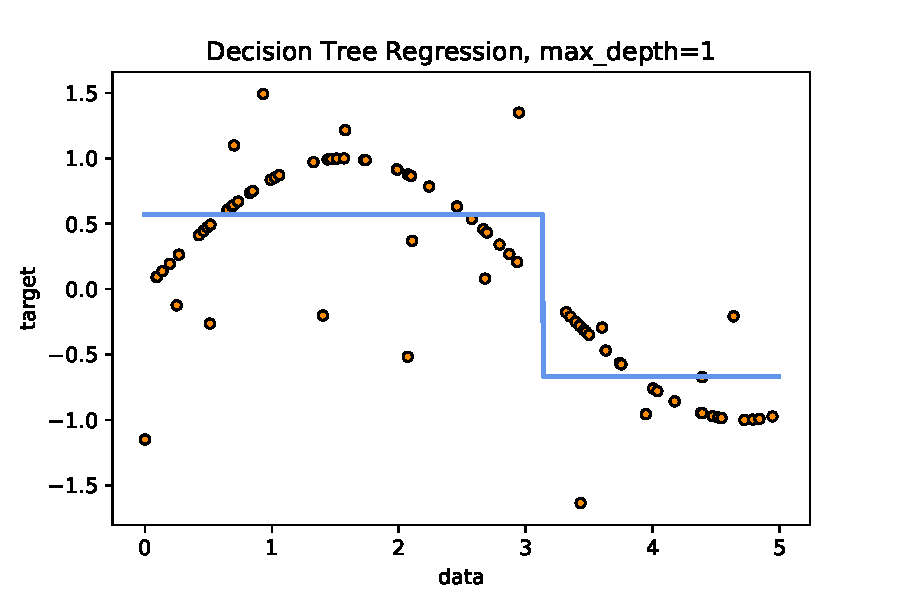
\includegraphics[width=0.47\linewidth]{figures/trees-sin-1.pdf}
\hfill
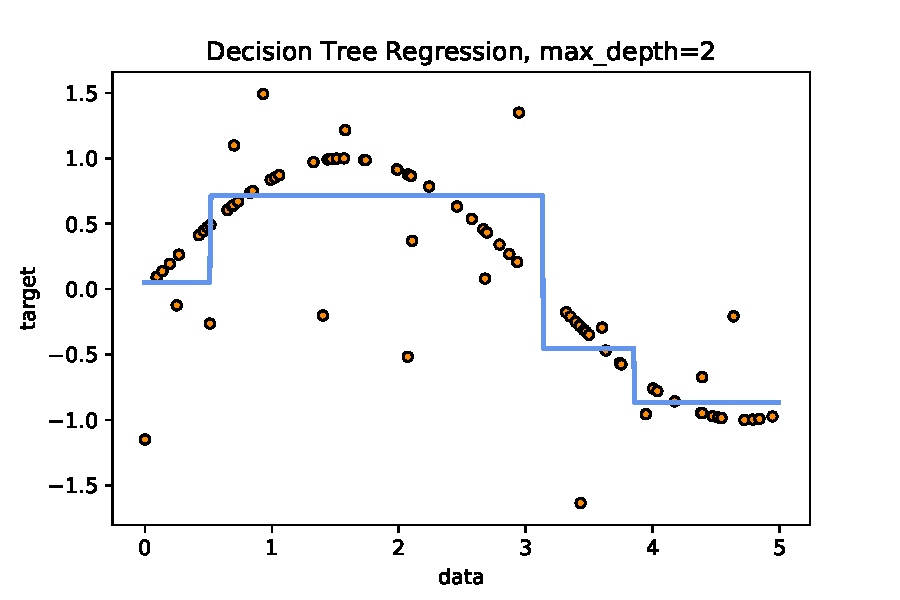
\includegraphics[width=0.47\linewidth]{figures/trees-sin-2.pdf}

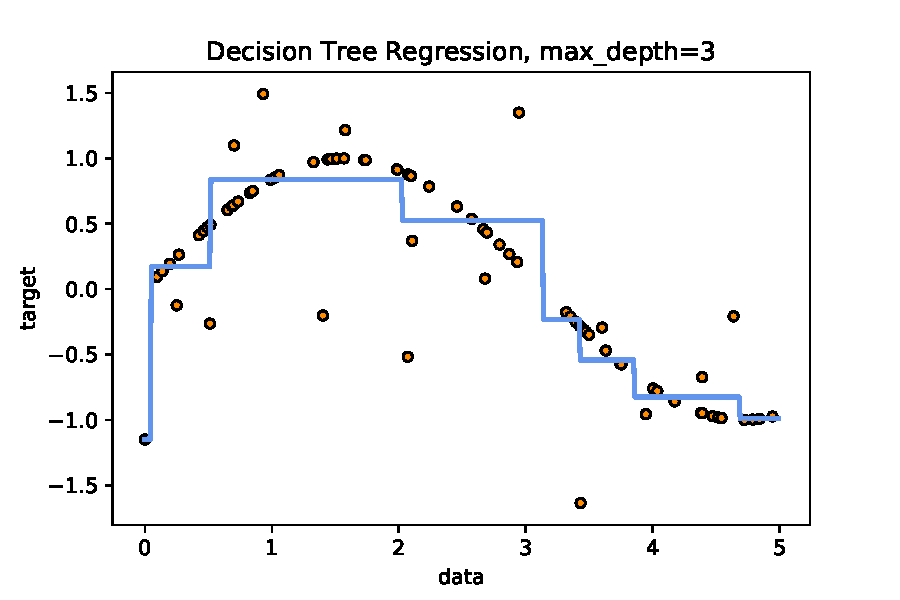
\includegraphics[width=0.47\linewidth]{figures/trees-sin-3.pdf}
\hfill
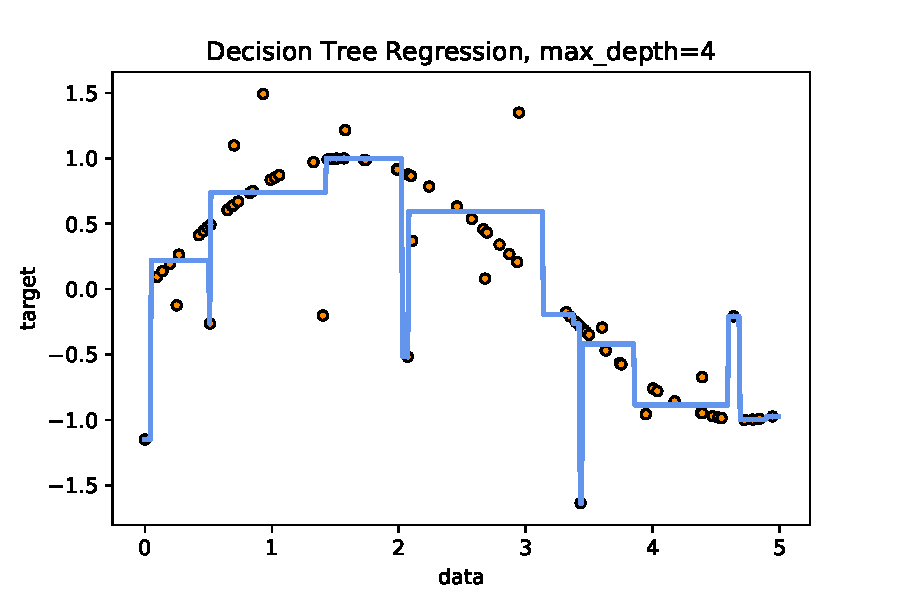
\includegraphics[width=0.47\linewidth]{figures/trees-sin-4.pdf}
}
\caption{Regression trees fitted on data generated by a sine function with some noise. While the tree adapts well to the training data, its ability to overfit the training data is visible already with trees with of maximum depth of 4 (lower right).}
\end{figure}

\begin{figure}[htbp]
\label{fig:fig:trees-sin-2}
\centering{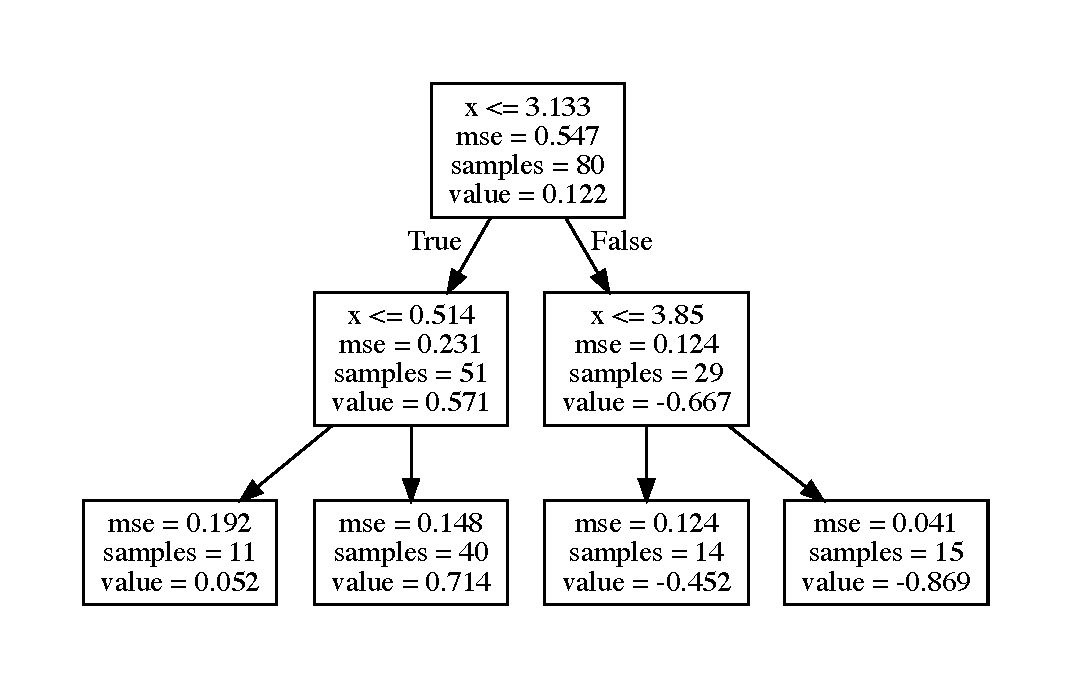
\includegraphics[width=0.7\linewidth]{figures/trees-rtree}}
\caption{A regression tree with maximum depth of 2 from the data from Fig.~\ref{fig:trees-sin}.}
\end{figure}


\ifguide{
This can be easily illustrated visually - linear models will work poorly on piecewise linear problems.
}

\subsection*{The CART algorithm}

Finding the optimal partitioning of the input variable space is in general NP-complete, even if using axis-parallel splits only. That is, it is infeasible to check all possible partitions. Instead, we will consider a greedy algorithm (CART) that is based on binary recursive partitioning of the input space, at each step choosing the best possible split (according to some pre-selected criterion). Notice that this algorithm does not use any look-ahead, and while such algorithms were studied in the literature, they are not used in practice. A simplified and abstracted CART algorithm is encoded as Algorithm~\ref{alg:cart}.

\ifguide{
I think Murphy's exposition of the algorithm could be better. And I don't understand what the anonymous function line is about. 
}

\begin{algorithm}
\caption{CART}\label{alg:cart}
\begin{algorithmic}[1]
\Procedure{fitTree}{data}
\State $(dataL, dataR, criterion) \gets split(data)$
\State $node \gets createNode(criterion, data)$
\If {(stoppingCriterionMet(...))} \Return node \EndIf
\State $node.L \gets fitTree(dataL)$
\State $node.R \gets fitTree(dataR)$
\State \Return node
\EndProcedure
\end{algorithmic}
\end{algorithm}

The CART algorithm uses several functions that require explanation:
\begin{itemize}
\item {\em createNode()}: This function creates an object that represents a tree node, which essentially stores the criterion on which the data in the node is split, and a possible reference to the data instances that are pertinent to the node. If a suitable node split is found, the node stores the information on its to siblings. Note that, as introduced above, the CART algorithm would construct binary trees.
\item {\em split()}: The assumption here is that features are numerical or at least ordinal. We order every feature based on possible splits (based on unique values in the data, so we have a finite number of possible splits). And then we basically go through all possible feature-split combinations to find the one that is optimal according to our splitting criterion - the one that minimizes the sum of the cost of the left and right subtrees. Possible splitting criterions are discussed below.

\item {\em stoppingCriterionMet()}: The stopping criterion can be one or more of the following:
\begin{itemize}
\item When the partition is sufficiently homogeneous/pure. In particular, there is no point in splitting further if we have perfect homogeneity (all observations have the same value).
\item When the gain (relative to stopping criterion) is smaller than some pre-determined threshold.
\item Reaching pre-determined maximum tree depth.
\item Reaching pre-determined minimum number of obvervations in a leaf.
\end{itemize}
\end{itemize}

\subsection*{Choice of the Splitting Criterion}
\end{document}

(purity, cost, loss, error)

**Numerical target variable:**

* The MSE of predicting with the subtree mean.

**Numerical target variable:**

* Misclassification rate
* Entropy
* Gini

<div class="alert alert-info">
  <strong>Note:</strong> This is what Murphy lists. I can't come up with a reason why misclassification rate should be used. Entropy and Gini give very similar results, but Entropy takes a bit more time to compute because of the log (not that it really makes a difference).
  
I'm not in favor of wasting time on mentioning information gain (= entropy).
</div>  

Note that with all the above criteria, splitting will never decrease the quality (it can leave it the same if it is already homogeneous). That is, we are computing training set performance and potentially overfitting the data. This is discussed further down.

### **Discussion** {-}

**Main advantages and disadvantages**:

* Decision trees are easy to interpret (in fact, according to most research, only behind decision tables and individual rules when it comes to non-expert users). This is somewhat marred by the fact that the common decision tree algorithms are very sensitive to changes in the inputs (a small change in the inputs can result in a substantially different tree). We can mitigate this by using bootstrapping to check if the algorithm produces stable trees before proceeding with interpretation. Also, learning a (stable) tree that mimics a more complex model such as a tree ensemble, neural network, etc. is one of the most common approaches to explaining how the complex model works.

* Low computational complexity of training and prediction (they scale well to large data sets).

* Compared to more complex methods (ensembles of trees, neural networks, etc.) they have a relatively poor inductive bias. That is, they won't perform the best (or close to) in terms of predictive quality on most practical problems. The two main issues are a **lack of smoothness** and **difficulty of capturing additive relationships**.

<div class="alert alert-info">
  <strong>Note:</strong> See ESL for two very nice subsections that further explain the two issues.
</div>  

**Categorical input variables**: When splitting a predictor having q possible unordered values, there are 2q−1 − 1 possible partitions of the q values into two groups, and the com-
putations become prohibitive for large q. 

For binary target variables we can order the predictor classes according to the
proportion falling in outcome class 1. Then we split this predictor as if it
were an ordered predictor. One can show this gives the optimal split, in
terms of cross-entropy or Gini index, among all possible 2q−1−1 splits. This
result also holds for a quantitative outcome and square error loss—the cat-
egories are ordered by increasing mean of the outcome. The proof for binary outcomes
is given in Breiman et al. (1984) and Ripley (1996); the proof for quantita-
tive outcomes can be found in Fisher (1958). For multicategory outcomes,
no such simplifications are possible, although various approximations have
been proposed (Loh and Vanichsetakul, 1988).

The partitioning algorithm tends to favor categorical predictors with
many levels q; the number of partitions grows exponentially in q, and the
more choices we have, the more likely we can find a good one for the data
at hand. This can lead to severe overfitting if q is large, and such variables
should be avoided.

Note that dummy (one-hot) coding of categorical variables can lead to the opposite problem of individual binary variables not being selected over numerical variables.

<div class="alert alert-info">
  <strong>Note:</strong> This is a slightly condensed version of the section on this from from ESL. With the addition of the problem of dummy coding.
</div>  

**Why Binary Splits?**: Rather than splitting each node into just two groups at each stage (as
above), we might consider multiway splits into more than two groups.While
this can sometimes be useful, it is not a good general strategy. The problem
is that multiway splits fragment the data too quickly, leaving insufficient
data at the next level down. Hence we would want to use such splits only
when needed. Since multiway splits can be achieved by a series of binary
splits, the latter are preferred.

<div class="alert alert-info">
  <strong>Note:</strong> Directly from ESL.
</div>  

**Handling missing values**: Suppose our data has some missing predictor values in some or all of the
variables. We might discard any observation with some missing values, but
this could lead to serious depletion of the training set. Alternatively we
might try to fill in (impute) the missing values, with say the mean of that
predictor over the nonmissing observations. For tree-based models, there
are two better approaches. The first is applicable to categorical predictors:
we simply make a new category for “missing.” From this we might dis-
cover that observations with missing values for some measurement behave
differently than those with nonmissing values. The second more general
approach is the construction of surrogate variables. When considering a
predictor for a split, we use only the observations for which that predictor
is not missing. Having chosen the best (primary) predictor and split point,
we form a list of surrogate predictors and split points. The first surrogate
is the predictor and corresponding split point that best mimics the split of
the training data achieved by the primary split. The second surrogate is
the predictor and corresponding split point that does second best, and so
on. When sending observations down the tree either in the training phase
or during prediction, we use the surrogate splits in order, if the primary
splitting predictor is missing. Surrogate splits exploit correlations between
predictors to try and alleviate the effect of missing data. The higher the cor-
relation between the missing predictor and the other predictors, the smaller
the loss of information due to the missing value.

<div class="alert alert-info">
  <strong>Note:</strong> Directly from ESL. I think this can be explained in more detail if time permits.
</div>  

**Tree pruning**: If the tree is allowed to grow until the leaves are completely (or nearly) homogenous, we are likely to be overfitting. In some cases that is actually desireable - we will see such an example later with random forests, where we want individual tree in the ensemble to be very biased. However, in most cases, it is not.

To prevent overfitting we can carefully tune the stopping criteria. However, growing the entire tree and then post-processing it by *pruning* certain branches can sometimes lead to better results. The basic idea is to check each split if not making that split would not result in a significant increase in error. Additionally, we can use cross-validation to prune based on an estimate of generalization error, making the process more robust. Note that cross-validation could (should) in theory also be used when growing the tree - the reason why we make splits based on what is essentially training set error is that cross-validation would be computationally infeasible in most practical scenarios. ... In some cases, it is, however, computationally feasible to use approximations to CV, such as AIC.

**Non-trivial models in the leaves**: Many approaches combine trees with generalized linear (additive) models in the leaves. This can lead to better results in problems that are a combination of crisp rules and (local) linear behavior, while retaining most of the interpretability. However, it comes at a cost of computational complexity, because it requires more complex model evaluation when splitting the tree.

**Axis-parallel partitioning**: Most tree-based algorithms (including the one described above) limit themselves axis-parallel splits. This can lead to very complicated trees if the boundaries between homogeneous regions do not follow this assumption. As an alternative, non axis-parallel (oblique) algorithms have been developed. However, this comes at a cost of interpretability and computational complexity.



\section{Bagging}

Before we proceed with random forests, we will first introduce a component of random forests what has more general applicability.

Bagging (Bootstrap Aggregation) is a general techique that can improve the predictive quality of models, in particular when the data set is small and/or we are dealing with a high-variance model (overfitting model), such as a non-pruned tree.

The basic idea is simple: instead of using our model $\hat{f}$ that was trained on all the training data, we make $B$ bootstrap replications of the training data and re-train the model on each, resulting in $B$ models $\hat{f}_b$. The bootstrapped prediction is the aggregate (average) of the individual bootstrap models:

$$\hat{f}_{\text{boot}}(x) = \sum_{b=1}^B \hat{f}_b(x).$$

In essence, we are using the bootstrap where the functional of the data is the model's prediction for $x$. And, as we already know, the sampling error can be made arbitrarily small by increasing B.

\subsection*{Why does it work?}

\ifguide{
Most of the arguments here are from Grandvalet, Y. (2004). Bagging equalizes influence. Machine Learning, 55(3), 251-270. Grandvalet provides a much better (and simpler) explanation than anything else I've seen.

Also note: Some authors (including ESL) say that the bagging estimate will be the same as the original model if the model is linear. That does not imply that bagging will produce the same estimate if used on linear regression.
}

There is little rigorous theoretical justification of why bagging should work, but there is ample empirical evidence that it often does work. Here we will offer some empirical justification for the underlying mechanisms that make bagging work (and sometimes fail):

Grandvalet (2004) argues that bagging equalizes the influence of individual points on the prediction. As the most influential points (points with high leverage) are typically outliers and have a bad influence on predictive quality, reducing their influence will improve performance (by reducing variance). This is a more general explanation to the more common explanation that bagging improves predictions because it reduces variance, in particular, because bagging can also increase variance. That is, if points of high leverage have a positive influence, bagging will decrease predictive quality.

One implication of the above is that models where all points have the same or similar leverage would not benefit from bagging. Similarly, models where a single point has very little effect on the prediction would also not benefit from bagging (robust models such as regularized regression or models that already contain some sort of bagging, such as random forests, which we discuss below). Therefore, high-variance models, such as non-pruned trees, is where we would expect the most benefit.


A prototypical example of where all points have the same leverage (and bagging does nothing) is predicting with the training set average. With enough bootstrap samples, every point will be included in the bootstrap sample approximately the same number of times and every point has the same influence. Indeed, the bootstrap prediction will be approximately the same as the prediction of the model that uses the entire training set.

In general, every point will be included in the bootstrap sample approximately the same number of times, but what is at first maybe even somewhat surprising, not every point has the same influence on the prediction. The fact that some points have more *leverage* on a prediction can be illustrated with simple linear regression, where points further away from the centre of mass (x-axis only) have more leverage. 

(green = true data generating process mean, black = lin. reg., red = bootstrapped lin. reg.)

Example 1: The outlier (bad point) is a high-leverage point hence bootstrapping improves performance.

![alt text here](./images/Rplot04.png)

Example 2: The outlier (bad point) is a low-leverage point. Bootstrapping gives it more influence, slightly decreasing performance.


![alt text here](./images/Rplot03.png)

Example 3: The outlier (this time it's a good point) is a high-leverage point. Bootstrapping gives it less influence, slightly decreasing performance.

![alt text here](./images/Rplot02.png)


\section{Random Forests}

* Basic idea: extend the idea of bagging to input variables as well: sampling input variables every step results in more decorrelated trees, but the variance of trees is still big, because we build them almost completely and we don't prune. Hence, they are ideal for bagging.
* Define the algorithm: ESL:Ch15.1 is good enough.
* Mention advantages: can be used for numeric and categorical target variable; elegant way of estimating generalization error (out-of-bag) and feature importance; very easy to tune
* Disadvantages: lose the interpretability of trees.

## Readings


* ESL:Ch09.2 (trees)
* Murphy:Ch16.2 (trees)
* ESL:Ch08.7 (bagging)
* ESL:Ch15.1 (random forests)


## Practice problem suggestions

* Implement a tree (to simplify, for continuous input variables only) with some stopping criterion and some variant of pruning. Test on a couple of simple datasets if better results can be achieved with pruning.
* Implement bagging of trees and compare with individual tree performance. Repeat same for a robust model.
